\documentclass[10pt,letterpaper,twocolumn]{article}
\usepackage[letterpaper,left=0.75in,right=0.75in,top=0.75in,bottom=1in,columnsep=24pt,headheight=12pt,headsep=22pt]{geometry}
\usepackage[T1]{fontenc}
\usepackage{mathptmx}
\renewcommand{\ttdefault}{pcr}
\usepackage{amsmath,booktabs,graphicx,array,float}
\usepackage{pgfplots}
\pgfplotsset{compat=1.18}
\usepgfplotslibrary{groupplots}
\usetikzlibrary{arrows.meta,positioning,calc}
\definecolor{figblue}{HTML}{0072B2}
\definecolor{figred}{HTML}{D55E00}
\definecolor{figgray}{HTML}{4D4D4D}
\usepackage[font=small,labelfont=bf,labelsep=colon]{caption}
\usepackage{balance}
\usepackage[hidelinks]{hyperref}
% Generated by generate_results.py; edit accepted source data only through review.
\newcommand{\PrimaryRows}{
4 & FCFS & 103.970 & 8,856 & 13.072 & 0.034 \\
4 & RR & 79.047 & 6,782 & 20.519 & 0.049 \\
4 & Main & 110.090 & 9,011 & 10.496 & 0.040 \\
8 & FCFS & 208.438 & 17,677 & 8.715 & 0.104 \\
8 & RR & 158.261 & 13,556 & 19.670 & 0.104 \\
8 & Main & 219.345 & 17,932 & 5.714 & 0.104 \\
16 & FCFS & 416.886 & 35,318 & 3.892 & 0.104 \\
16 & RR & 316.614 & 27,102 & 18.694 & 0.095 \\
16 & Main & 437.623 & 35,773 & 1.158 & 0.084 \\
}
\newcommand{\OverheadRows}{
4 & 5.89 & 39.27 & 1132.0 & 263.0 & 7144.0 \\
8 & 5.23 & 38.60 & 2767.6 & 512.9 & 13596.4 \\
16 & 4.97 & 38.22 & 6038.5 & 1268.7 & 26673.2 \\
}
\newcommand{\AreaFCFS}{(4,103.970058316) (8,208.437730604) (16,416.886135213)}
\newcommand{\PolicyFCFS}{(4,1.131957400) (8,2.767628100) (16,6.038461400)}
\newcommand{\SetupFCFS}{(4,13.071612000) (8,8.714740000) (16,3.891612000)}
\newcommand{\AreaRR}{(4,79.047172316) (8,158.260808962) (16,316.614126327)}
\newcommand{\PolicyRR}{(4,0.263039000) (8,0.512862600) (16,1.268686900)}
\newcommand{\SetupRR}{(4,20.519341000) (8,19.669725000) (16,18.694050000)}
\newcommand{\AreaMain}{(4,110.089845892) (8,219.344574607) (16,437.622506788)}
\newcommand{\PolicyMain}{(4,7.143987900) (8,13.596449900) (16,26.673175400)}
\newcommand{\SetupMain}{(4,10.496409000) (8,5.713676000) (16,1.158148000)}
\newcommand{\ColdPowerRows}{
4 & FCFS & 3.397 & 3.399 & 3.398 & 116.9 \\
4 & RR & 2.600 & 2.602 & 2.600 & 89.5 \\
4 & Main & 3.500 & 3.501 & 3.500 & 120.5 \\
8 & FCFS & 6.728 & 6.729 & 6.725 & 222.4 \\
8 & RR & 5.175 & 5.175 & 5.173 & 171.0 \\
8 & Main & 6.924 & 6.924 & 6.920 & 228.9 \\
16 & FCFS & 13.4 & 13.4 & 13.4 & 441 \\
16 & RR & 10.3 & 10.3 & 10.3 & 339 \\
16 & Main & 13.8 & 13.8 & 13.8 & 454 \\
}
\newcommand{\ColdMeanFCFS}{(4,3.398) (8,6.727) (16,13.400)}
\newcommand{\ColdSeedsFCFS}{(3.76,3.397) (4.00,3.399) (4.24,3.398) (7.76,6.728) (8.00,6.729) (8.24,6.725) (15.76,13.400) (16.00,13.400) (16.24,13.400)}
\newcommand{\ColdMeanRR}{(4,2.601) (8,5.174) (16,10.300)}
\newcommand{\ColdSeedsRR}{(3.76,2.600) (4.00,2.602) (4.24,2.600) (7.76,5.175) (8.00,5.175) (8.24,5.173) (15.76,10.300) (16.00,10.300) (16.24,10.300)}
\newcommand{\ColdMeanMain}{(4,3.500) (8,6.923) (16,13.800)}
\newcommand{\ColdSeedsMain}{(3.76,3.500) (4.00,3.501) (4.24,3.500) (7.76,6.924) (8.00,6.924) (8.24,6.920) (15.76,13.800) (16.00,13.800) (16.24,13.800)}
\newcommand{\BoundaryRows}{
FCFS & 1.309 & 0.01912 & 2.056 & 3.383 & 153.5 \\
RR & 1.001 & 0.01453 & 1.570 & 2.586 & 117.3 \\
Main & 1.334 & 0.02043 & 2.141 & 3.495 & 158.6 \\
}
\newcommand{\BoundaryInternal}{(1,1.309) (2,1.001) (3,1.334)}
\newcommand{\BoundarySwitching}{(1,0.01912) (2,0.01453) (3,0.02043)}
\newcommand{\BoundaryLeakage}{(1,2.056) (2,1.570) (3,2.141)}
\newcommand{\SupplementRows}{
Total area (library units) & 110089.846 & 110058.332 \\
Policy subtree area & 7143.988 & 7120.861 \\
Flip-flop cells & 9,011 & 9,011 \\
Setup slack (ns) & 10.496409 & 10.547482 \\
Hold slack (ns) & 0.039940 & 0.039940 \\
Constant-disabled checks & 68 & 68 \\
}

% v3 only; generated from pinned accepted evidence. Do not edit.

\newcommand{\RevisionMatrixPassed}{498}

\newcommand{\RevisionMatrixPlanned}{498}

\newcommand{\RevisionConfirmationTable}{%
\begin{tabular}{llrrrr}
\hline
Policy & High:Low & A P99 & B P99 & A mean & B mean \\
\hline
FCFS & -- & 18.10 & 33.45 & 16.392 & 23.306 \\
RR1 & -- & 2.00 & 16.65 & 1.025 & 8.129 \\
RR10 & -- & 11.00 & 17.70 & 5.584 & 9.153 \\
FAI-inspired & -- & 10.00 & 21.05 & 5.522 & 9.240 \\
Algorithm-2 & -- & 10.00 & 21.35 & 5.525 & 9.326 \\
BLISS-inspired & -- & 1.15 & 33.00 & 1.009 & 21.696 \\
CGOF (2:1) & 2:1 & 1.10 & 12.35 & 1.008 & 6.092 \\
\hline
\end{tabular}%
}

\newcommand{\RevisionPninetyNineA}{(1,18.10) (2,2.00) (3,11.00) (4,10.00) (5,10.00) (6,1.15) (7,1.10)}

\newcommand{\RevisionPninetyNineB}{(1,33.45) (2,16.65) (3,17.70) (4,21.05) (5,21.35) (6,33.00) (7,12.35)}

\newcommand{\RevisionPairedCITable}{%
\begin{tabular}{lllrr}
\hline
Candidate / baseline & High:Low & Arm & $\Delta$ P99 & 95\% CI \\
\hline
FAI-inspired / FCFS & -- & A & -8.10 & [-8.25, -8.00] \\
FAI-inspired / FCFS & -- & B & -12.40 & [-13.25, -11.55] \\
FAI-inspired / RR10 & -- & A & -1.00 & [-1.00, -1.00] \\
FAI-inspired / RR10 & -- & B & 3.35 & [2.25, 4.45] \\
CGOF (2:1) / FAI-inspired & 2:1 & A & -8.90 & [-9.00, -8.75] \\
CGOF (2:1) / FAI-inspired & 2:1 & B & -8.70 & [-9.50, -7.90] \\
\hline
\end{tabular}%
}

\newcommand{\RevisionNExpansionTable}{%
\begin{tabular}{rlrrrr}
\hline
N & Policy & A P99 & B P99 & A mean & B mean \\
\hline
8 & FCFS & 20.00 & 37.60 & 16.945 & 23.995 \\
8 & RR1 & 2.00 & 20.20 & 1.059 & 8.387 \\
8 & RR10 & 12.00 & 21.00 & 5.799 & 9.423 \\
8 & FAI-inspired & 10.00 & 27.60 & 5.552 & 9.797 \\
8 & Algorithm-2 & 10.00 & 28.20 & 5.500 & 9.792 \\
8 & BLISS-inspired & 2.00 & 37.00 & 1.025 & 22.213 \\
16 & FCFS & 22.00 & 41.80 & 18.174 & 25.437 \\
16 & RR1 & 3.00 & 23.40 & 1.134 & 8.956 \\
16 & RR10 & 13.00 & 24.40 & 6.174 & 10.055 \\
16 & FAI-inspired & 10.00 & 34.80 & 5.562 & 11.094 \\
16 & Algorithm-2 & 10.00 & 35.20 & 5.565 & 11.205 \\
16 & BLISS-inspired & 2.00 & 41.60 & 1.063 & 23.506 \\
\hline
\end{tabular}%
}

\newcommand{\RevisionPowerTable}{%
\begin{tabular}{llrrrr}
\hline
Policy & Arm & Internal & Switching & Leakage & Total \\
\hline
FCFS & A & 1.306000 & 0.017807 & 2.032000 & 3.356000 \\
FCFS & B & 1.306000 & 0.017547 & 2.033000 & 3.356000 \\
RR10 & A & 0.999500 & 0.013447 & 1.546667 & 2.559667 \\
RR10 & B & 0.999100 & 0.013090 & 1.548000 & 2.560000 \\
FAI-inspired & A & 1.331667 & 0.019203 & 2.116000 & 3.466667 \\
FAI-inspired & B & 1.331000 & 0.018737 & 2.116667 & 3.466000 \\
\hline
\end{tabular}%
}

\newcommand{\RevisionCgofPpaTable}{%
\begin{tabular}{lrrrrrr}
\hline
High:Low & Cell area & Registers & Setup ns & Hold ns & Untested & Formal points \\
\hline
2:1 & 109794.784709 & 9014 & 10.398800 & 0.038578 & 68 & 9126 \\
\hline
\end{tabular}%
}

% N4 subset of the full nine-case disjoint leaf audit; square micrometres; printed rounding applies.
\newcommand{\RevisionPrimaryAreaTable}{%
\begin{tabular}{lrrrrrr}
\hline
N4 policy & Descriptor & Timestamp & Policy logic & Common & Residual & Whole area \\
\hline
FCFS & 44404.041137 & 13532.660156 & 1131.957370 & 44901.399654 & -0.000001002 & 103970.058316 \\
RR10 & 44404.041137 & 0.000000 & 263.039041 & 34380.092136 & 0.000002003 & 79047.172316 \\
FAI-inspired & 44404.041139 & 13532.660157 & 7143.987889 & 45009.156711 & -0.000002999 & 110089.845892 \\
\hline
\end{tabular}%
}

\newcommand{\RevisionFaiOverRRMin}{38.22}

\newcommand{\RevisionFaiOverRRMax}{39.27}

\newcommand{\RevisionRRBelowFaiMin}{27.65}

\newcommand{\RevisionRRBelowFaiMax}{28.20}

% Generated from completed, hash-bound October 28 evidence; no new experiment.

% MODEL_ONLY P99 is mean per-run pooled-Sparse G-to-F P99, including completed cleanup requests.

% MODEL_ONLY Heavy gap is mean per-run maximum uncensored FIFO-nonempty inter-service wall-cycle gap.

% W5M is configured; the short model controls end BEFORE the first classification boundary.

\newcommand{\ImprovementCgofHardwareTable}{%
\begin{tabular}{lrrrr}
\hline
Policy & N & Cell area & Setup (ns) & Hold (ns) \\
\hline
CGOF (1:1) & 4 & 106163.066946 & 12.683299 & 0.034898 \\
CGOF (1:1) & 8 & 212027.006396 & 8.135937 & 0.054674 \\
CGOF (1:1) & 16 & 423513.448454 & 3.158005 & 0.078278 \\
CGOF (2:1) & 4 & 109794.784709 & 10.398800 & 0.038578 \\
CGOF (2:1) & 8 & 218863.734160 & 5.675092 & 0.103860 \\
CGOF (2:1) & 16 & 436771.124393 & 1.248813 & 0.084335 \\
\hline
\end{tabular}%
}

\newcommand{\ImprovementFixedClassTable}{%
\begin{tabular}{lrrrr}
\hline
Policy & Low 0 (\%) & High 1 (\%) & High 2 (\%) & High 3 (\%) \\
\hline
FAI-inspired & 49.9975 & 16.6708 & 16.6658 & 16.6658 \\
CGOF (1:1) & 25.0013 & 25.0013 & 25.0013 & 24.9962 \\
CGOF (2:1) & 14.2857 & 28.5714 & 28.5714 & 28.5714 \\
\hline
\end{tabular}%
}

\newcommand{\ImprovementFiniteHeavyModelTable}{%
\begin{tabular}{lrrr}
\hline
Policy & Sparse P99 & Heavy max gap & Completion ratio \\
\hline
FAI-inspired & 28.30 & 7.00 & 1.2002146 \\
CGOF (1:1) & 4.15 & 7.55 & 1.2004486 \\
CGOF (2:1) & 4.85 & 9.55 & 1.2004373 \\
WRR (2:1) & 10.00 & 7.35 & 1.2003968 \\
IWRR (2:1) & 8.70 & 7.35 & 1.2004261 \\
\hline
\end{tabular}%
}

% Production RTL: near profile, seed 6201, Heavy work 5,000,000; one B_H/H/H/H boundary, all effective High.

\newcommand{\ImprovementProductionRtlTable}{%
\begin{tabular}{lrrr}
\hline
Policy & Sparse P99 & Heavy max gap & Completion ratio \\
\hline
CGOF (1:1) & 3 & 9 & 1.00000048 \\
CGOF (2:1) & 4 & 10 & 1.00000048 \\
\hline
\end{tabular}%
}

% Generated by generate_update_20261029.py; all values in cycles.
\newcommand{\UpdateFiniteHeavyTable}{%
\begin{tabular}{lrrr}\toprule
High:Low & Sparse run-P99 & Heavy run maximum gap & Heavy completion delay \\\midrule
1:1 & 3.00 [3.00, 3.00] & 9.45 [9.15, 9.75] & 3.05 [1.45, 5.05] \\
2:1 & 4.00 [4.00, 4.00] & 10.85 [10.45, 11.35] & 3.00 [1.40, 5.00] \\
\bottomrule\end{tabular}}
\newcommand{\UpdatePerformanceTable}{%
\begin{tabular}{llcrr}\toprule
Stage & Sink readiness & Seeds & A Sparse run-P99 & B Sparse run-P99 \\\midrule
Confirmation & Always & 20 & 1.10 [1.00, 1.25] & 12.35 [11.80, 12.90] \\
Exploration & Bernoulli 0.75 & 5 & 5.00 & 20.40 \\
Exploration & Periodic 48/64 & 5 & 17.00 & 27.00 \\
\bottomrule\end{tabular}}

% Generated by generate_update_20261102.py from frozen manifests; do not edit manually.
\newcommand{\NovOrderingTable}{%
\begin{tabular}{@{}llrrrrr@{}}\toprule
Campaign (scope) & Metric & Q1-OF & Q1-RR & Q2-OF & Q2-RR & Contrast / verdict \\\midrule
W256 RTL ($n=20$ seeds, 160 jobs) & Sparse P99 $\Delta$ ($d_1, d_2$) & ref & $0.00$ & ref & $-0.35$ & $I=-0.35$ (7/20 $\le -1$; \code{NOT\_CONFIRMED}) \\
W256 RTL ($n=20$ seeds, 160 jobs) & Heavy max gap $\Delta$ & ref & $+0.00$ & ref & $-0.10$ & 0/20 Q1 diff; 2/20 Q2 diff \\
W5M RTL ($n=5$ seeds, 40 jobs) & Sparse G$\to$F P99 & $11$ & $11$ & $12$ & $11$ & $d_1=0, d_2=-1, I=-1$ (5/5 seeds) \\
W5M RTL ($n=5$ seeds, 40 jobs) & Heavy max gap $\Delta$ & ref & $+1.6$ & ref & $-0.2$ & Q1: $+2,+2,+1,+2,+1$; Q2: $0,0,0,0,-1$ \\
W5M RTL ($n=5$ seeds, 40 jobs) & Extra completion $A$ $\Delta$ & ref & $0.0$ & ref & $0.0$ & $A=3,0,7,1,8$ cycles; RR$-$OF $=0$ (10/10) \\
\bottomrule\end{tabular}}

\newcommand{\NovArrivalSlackTable}{%
\begin{tabular}{@{}llrrrr@{}}\toprule
Cohort (MODEL\_ONLY) & Load & Mixed$-$isolated $\Delta C$ (cycles) & Time ratio & Mean max lag (desc.) & Recovery / margin \\\midrule
W5M confirmation ($n=20$) & Under & $0.00$ $[0.0, 0.0]$ & $1.000000$ & -- & 20/20 in $\pm 20$c \\
W5M confirmation ($n=20$) & Over & $834.25$ $[820.4, 849.3]$ & $1.037553$ & -- & 0/20 in $\pm 20$c \\
W256 P0 common-$H$ ($20$ obs.) & Under & $0.00$ & $1.000000$ & $1.25$ / $1.25$ & 20/20 rec.; 20/20 margin \\
W256 P0 common-$H$ ($20$ obs.) & Near & $0.00$ & $1.000000$ & $5.00$ / $4.95$ & 20/20 rec.; 20/20 margin \\
W256 P0 common-$H$ ($20$ obs.) & Over & $85.20$ & $1.149956$ & $75.60$ / $75.60$ & 20/20 rec.; 0/20 margin \\
\bottomrule\end{tabular}}

\newcommand{\NovDynamicProbeTable}{%
\begin{tabular}{@{}llrrrrrr@{}}\toprule
Case (seed 7291, W5M) & Policy & Boundaries / flips & Sparse P99 & Heavy G$\to$A / A$\to$F / G$\to$F P99 & Wall gap P99/max & Ready gap P99/max & $\Delta C$ \\\midrule
Multi-window (D16) & CGOF (1:1) & 4 / 1 & 3 & 4 / 19 / 22 & 3 / 10 & 2 / 4 & +5 \\
Multi-window (D16) & CGOF (2:1) & 4 / 1 & 4 & 3 / 19 / 22 & 3 / 11 & 2 / 7 & +5 \\
Role switch (D16) & CGOF (1:1) & 4 / 3 & 3 & 4 / 19 / 22 & 3 / 9 & 2 / 4 & +6 \\
Role switch (D16) & CGOF (2:1) & 4 / 3 & 4 & 4 / 19 / 22 & 3 / 11 & 2 / 7 & +6 \\
Ready spread (D16) & CGOF (1:1) & 4 / 1 & 3 & 0 / 16 / 16 & 3 / 5 & 2 / 4 & +4 \\
Ready spread (D16) & CGOF (2:1) & 4 / 1 & 3 & 0 / 16 / 16 & 3 / 8 & 2 / 7 & +4 \\
Ready bursty (D16) & CGOF (1:1) & 4 / 1 & 11 & 2 / 18 / 20 & 11 / 14 & 2 / 4 & +5 \\
Ready bursty (D16) & CGOF (2:1) & 4 / 1 & 11 & 2 / 18 / 20 & 11 / 17 & 2 / 7 & +5 \\
Ready bursty (D8) & CGOF (1:1) & 4 / 1 & 11 & 11 / 16 / 20 & 11 / 14 & 2 / 4 & +5 \\
Ready bursty (D8) & CGOF (2:1) & 4 / 1 & 11 & 11 / 16 / 20 & 11 / 17 & 2 / 7 & +5 \\
\bottomrule\end{tabular}}

\pdfinfoomitdate=1
\pdfsuppressptexinfo=-1
\pdftrailerid{}
\hypersetup{pdftitle={From Service Classes to Hardware Costs: An RTL Study of CXL-Inspired Switch Scheduling},pdfauthor={Jay Chiang; Daniel Chou},pdfsubject={ECE 509 final report; completed evidence through 2026-11-02}}
\setlength{\parindent}{1em}
\setlength{\parskip}{0pt}
\setlength{\textfloatsep}{8pt plus 2pt minus 2pt}
\setlength{\floatsep}{7pt plus 2pt minus 2pt}
\setlength{\intextsep}{8pt plus 2pt minus 2pt}
\renewcommand{\dbltopfraction}{0.88}
\renewcommand{\textfraction}{0.10}
\renewcommand{\dblfloatpagefraction}{0.75}
\setcounter{dbltopnumber}{3}
\setlength{\abovedisplayskip}{4pt plus 1pt minus 1pt}
\setlength{\belowdisplayskip}{4pt plus 1pt minus 1pt}
\setlength{\abovedisplayshortskip}{2pt plus 1pt}
\setlength{\belowdisplayshortskip}{2pt plus 1pt}
\setlength{\headheight}{12pt}
\setlength{\emergencystretch}{1.3em}
\clubpenalty=10000
\widowpenalty=10000
\brokenpenalty=10000
\raggedbottom
\newcolumntype{P}[1]{>{\raggedright\arraybackslash}p{#1}}
\makeatletter
\renewcommand{\section}{\@startsection{section}{1}{\z@}{-2.6ex plus -0.6ex minus -0.2ex}{1.1ex plus 0.2ex}{\normalfont\large\bfseries\raggedright}}
\renewcommand{\subsection}{\@startsection{subsection}{2}{\z@}{-2.2ex plus -0.5ex minus -0.2ex}{0.8ex plus 0.2ex}{\normalfont\normalsize\bfseries\raggedright}}
\def\ps@report{%
  \def\@oddhead{\footnotesize CXL Switch Arbitration: Policy to Hardware Cost\hfil Chiang and Chou}%
  \let\@evenhead\@oddhead
  \def\@oddfoot{\hfil\footnotesize\thepage\hfil}%
  \let\@evenfoot\@oddfoot}
\makeatother
\pagestyle{report}
\newcommand{\FaiInspired}{FAI-inspired}
\newcommand{\Alg}{FAI-ImmBuf}
\newcommand{\code}[1]{\texttt{#1}}
\newcommand{\reportaxis}{\pgfplotsset{every axis/.append style={width=\columnwidth,height=4.25cm,scale only axis=false,tick label style={font=\scriptsize,text=figgray},label style={font=\scriptsize,text=figgray},legend style={font=\scriptsize,draw=none,fill=white,inner sep=1pt},grid=major,grid style={figgray!15,line width=.25pt},axis line style={figgray!70,line width=.45pt},tick style={figgray!70,line width=.4pt},xmin=2.5,xmax=17.5,xtick={4,8,16},xlabel={Number of sources $N$},axis x line=bottom,axis y line=left}}}
\title{\vspace{-2em}\bfseries From Service Classes to Hardware Costs:\\ An RTL Study of CXL-Inspired Switch Scheduling}
\author{Jay Chiang\qquad Daniel Chou}
\date{\normalsize ECE 509 Final Project Report\\\small Revised November 2, 2026 (Asia/Taipei)}
\begin{document}
\maketitle
\begin{abstract}
Memory pooling allows hosts to share remote memory capacity while concentrating requests on shared service paths. We study how service-history classification and service allocation shape waiting in a single-output register-transfer-level (RTL) switch inspired by Compute Express Link (CXL). A common descriptor, queue, and output contract supports comparisons of first-come-first-served, round-robin, FAI-inspired class arbitration, and per-source Credit-Gated Oldest-First (CGOF) scheduling. Across twenty confirmation seeds with four sources (N4), FAI-inspired reduces mean per-run 99th-percentile (P99) generation-to-fire delay of intermittent (Sparse) requests from 18.10 to 10.00 cycles for independent arrivals and from 33.45 to 21.05 for bursts; round-robin with quantum ten reaches 17.70 cycles for bursts. A current-source CGOF (2:1) replay reproduces 1.10/12.35 cycles. Fixed-class models explain the distinct shares produced by class quotas and per-source credits. A separate twenty-seed finite-work RTL confirmation crosses one production classification boundary: CGOF (1:1)/(2:1) gives Sparse P99 of 3/4 cycles and mean per-run maximum Heavy service gap of 9.45/10.85 cycles, while mixed Heavy completion averages 3.05/3.00 cycles longer than isolated execution. Equal relative weights can thus coexist with different short-term service patterns as absolute credit budgets change. Follow-up quota-by-ordering RTL experiments show that eligible round-robin ordering is not confirmed as a universal improvement at W256 (7/20 seeds, mean $-0.35$ cycle) and trades a one-cycle Q2 Sparse P99 reduction ($12\rightarrow 11$ cycles, $I=-1$) against a $+1.6$-cycle mean Q1 maximum Heavy gap in five-seed W5M production runs. Six CGOF mappings meet evaluated timing checks at 25\,ns for four, eight, and sixteen sources; N4 CGOF (2:1) has 0.268\% less complete cell area than FAI-inspired. These results connect allocation, service regularity, and implementation cost at a reproducible scheduler boundary.
\end{abstract}

\section{CXL Pooling and Shared-Path Contention}
\label{sec:pooling}
Memory tied to individual servers can remain unused even when other servers need additional capacity. Compute Express Link (CXL) pooling offers a way to make that capacity available across hosts. Pond motivates pooling through memory stranding and couples the hardware opportunity with placement decisions that account for access latency~\cite{pond}. CXL's memory semantics allow processors to access pool memory through cacheable loads and stores, giving software a familiar interface to physically remote capacity~\cite{cxl_intro}. Capacity utilization and access performance are therefore closely connected design concerns.

The path to pooled memory introduces shared points of contention. Requests from several hosts can converge on a switch egress, a downstream link, or a memory device. Even when an output remains continuously busy, its arbitration policy determines whose requests advance and whose requests accumulate. Placement and interleaving determine which resources requests reach; scheduling determines how competing requests share a resource once they arrive. Systems such as Pond, Transparent Page Placement, and DirectCXL address complementary parts of this problem~\cite{pond,tpp,directcxl}. Pooling economics and topology choices further affect the useful operating region~\cite{case_pool,my_cxl_pool}.

\begin{figure*}[t]
\centering
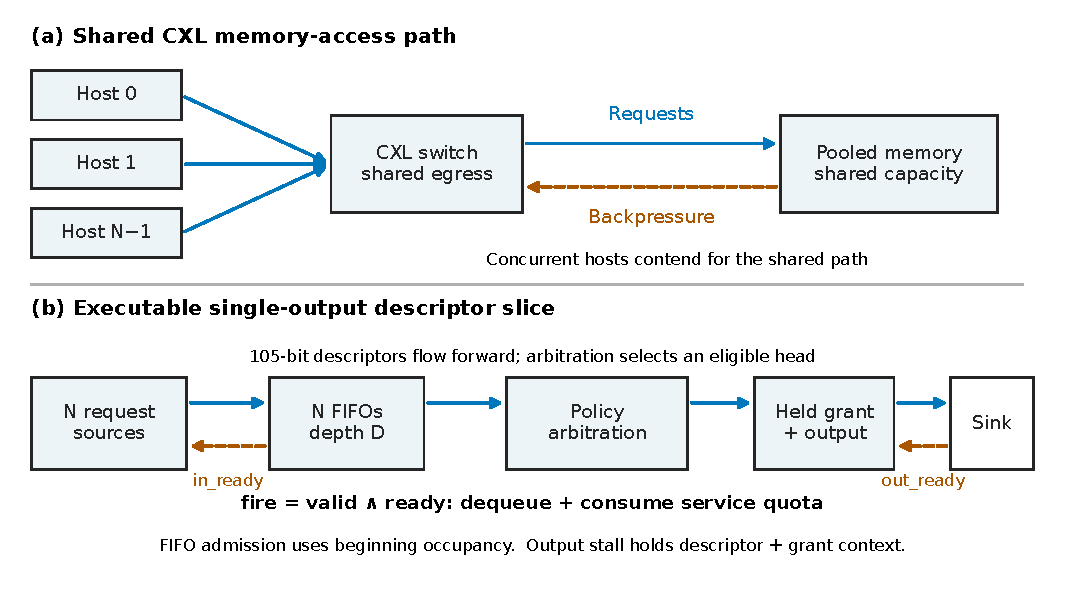
\includegraphics[width=\textwidth]{generated/figures/improvement/pooling-path.pdf}
\caption{Conceptual pooled-memory access path and the evaluated single-output slice. CXL memory access motivates the host--switch--memory path~\cite{cxl_intro,pond,fai}; the inset specifies this project's per-source first-in-first-out (FIFO) request queues and shared output. The slice transports equal-cost 105-bit descriptors, one per successful output opportunity.}
\label{fig:pooling}
\end{figure*}

Consider one source that continuously offers work and three that issue occasional requests. We call these workload roles \emph{Heavy} and \emph{Sparse}. A Heavy source can keep an output occupied while a newly active Sparse source waits behind previously admitted work. Giving the Sparse source earlier service can reduce its tail without increasing total output throughput. The same decision can also change the intervals between Heavy services. Aggregate throughput alone consequently provides an incomplete account of interference. Figure~\ref{fig:pooling} locates the arbitration boundary at which these effects can be examined directly.

This boundary shares familiar properties with packet switches: finite service capacity, queues, arbitration, and backpressure. Fixed-cost internal transfers also appear in packet-switch designs, including the fixed-size cells used by Gupta and McKeown~\cite{gupta}. In pooled memory, arbitration lies on the path that supplies data to processor memory operations, so queueing can delay dependent computation. This connects memory-service interference to the hardware cost of scheduling at a shared path~\cite{cxl_intro,stfm}. We represent the shared path as one output with per-source queues, making the service rules explicit enough to implement and compare cycle by cycle. System-level interference, caching, and memory behavior motivate subsequent integration with the broader CXL studies and simulators~\cite{cxl_interplay,contention_cache,hpc_pool,cxldmsim}.

We ask how recent service becomes a priority decision, how that priority becomes an allocation of service opportunities, and what complete hardware cost implements those choices. FAI-CXL provides the starting point: its scheduler classifies hosts by recent service and introduces a transitional Buffer state~\cite{fai}. We reconstruct that mechanism in executable RTL, compare it against simpler policies on a common platform, and use allocation controls to explain the resulting latency patterns. The evaluation joins scheduler models, register-transfer-level (RTL) execution, and pre-layout implementation measurements, with each answering a different part of the design question.

The resulting argument is that classification, allocation, and request ordering must be examined together. A priority class acquires operational meaning through its allocated service quota and the sources competing for that quota. Tail improvements likewise acquire practical meaning when paired with service-gap and hardware-cost measurements. This study supplies those connections for the specified descriptor switch, beginning with the purpose of FAI's service-history mechanism.

\section{FAI: Service History, Priority, and Transitional Buffer}
\label{sec:fai}
FAI-CXL (Fairness-Aware Interleaved CXL) combines a unified pool manager, cacheline-level weighted interleaving, and adaptive scheduling~\cite{fai}. Its interleaver distributes addresses across memory devices; its scheduler addresses contention among hosts using those devices. The scheduler observes service over a fixed window, identifies relatively low- and high-service hosts, and adjusts their priority. This distinction matters in the Heavy/Sparse example: the classifier observes the service a host actually receives, which is shaped jointly by arrivals, admission, and prior scheduling decisions.

For each source $h$, let $B[h]$ count successful services within a window and let $S=\sum_h B[h]$. The average is $S/N$ over all $N$ configured sources, including inactive ones. With threshold $\theta=0.3$, a host receiving less than 30\% of the average generates UP evidence; one receiving more than the average generates DOWN evidence. Intermediate values, including equality, generate KEEP. The division-free form used in this project is
\begin{align}
\mathrm{UP}:&\quad 10NB[h]<3S,\nonumber\\
\mathrm{DOWN}:&\quad NB[h]>S,\label{eq:class-v3}\\
\mathrm{KEEP}:&\quad\text{otherwise}.\nonumber
\end{align}
These comparisons estimate relative delivered service. They need no prediction of future arrivals or access to work still waiting in an external producer.

The transitional Buffer state provides a time interval between evidence for a change and commitment to an effective priority. In our primary \emph{FAI-inspired} interpretation, called Main below, the states are $H$, $B_H$, $L$, and $B_L$. Both $H$ and $B_H$ receive High-class service; both $L$ and $B_L$ receive Low-class service. Starting in $H$, a DOWN window produces $B_H$. A second consecutive DOWN produces $L$. Conversely, two consecutive UP windows move $L\rightarrow B_L\rightarrow H$. Thus the first supporting window records a pending decision while preserving the current service class.

\begin{figure*}[t]
\centering
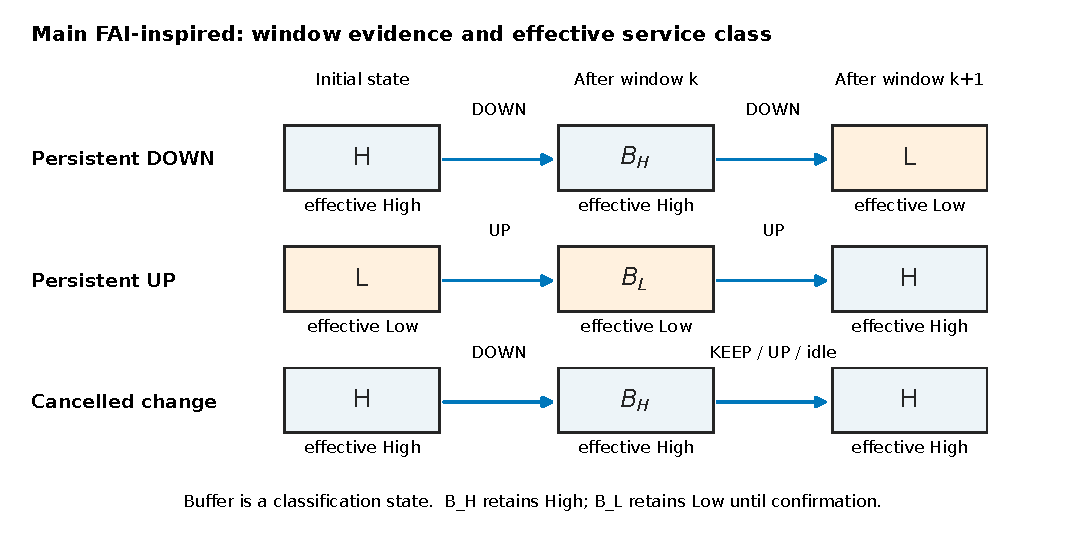
\includegraphics[width=\textwidth]{generated/figures/improvement/buffer-transition.pdf}
\caption{Main's transitional Buffer semantics, specified in the project contract~\cite{artifact}. Two successive supporting windows change effective class. $B_H$ remains High and $B_L$ remains Low; KEEP, opposing evidence, or an idle window cancels the pending transition. Buffer is classifier state, separate from the request FIFOs.}
\label{fig:buffer}
\end{figure*}

Figure~\ref{fig:buffer} shows why this is a hysteresis mechanism. A single DOWN observation followed by KEEP gives \mbox{$H\rightarrow B_H\rightarrow H$}, with High service throughout. An idle window also cancels a pending transition. The corresponding Low sequence behaves symmetrically. A sustained change requires an additional confirming window, trading responsiveness for resistance to isolated observations. This is a property of the transition rule; its effect on waiting depends on when workload changes occur and how the allocation mechanism uses the resulting classes.

The FAI-CXL paper contains two descriptions that lead to different executable rules. Section IV-C describes Buffer as retaining the previous priority for one window. In Algorithm 2, lines 13 and 18 instead assign the target priority to $P_{\rm last}$ on entry to Buffer, and lines 4--5 use that value for dispatch~\cite{fai}. We retain both interpretations. Main implements previous-effective-class hysteresis. For readability, we call the supplementary immediate-target Buffer reconstruction \emph{\Alg} (labelled \code{Algorithm-2} in archived evidence artifacts): it serves a Buffer host immediately in its stored target class and retains Buffer on KEEP or an idle window. Both use the same thresholds and project-defined single-output 10/10 class alternation.

This explicit separation makes the comparison interpretable. Heavy/Sparse names describe traffic, whereas High/Low names describe the service classes assigned during execution. A Heavy source may initially be High, and a pending downward transition may still receive High service. Likewise, a FIFO stores requests while Buffer stores a classification decision. With these meanings fixed, the next step is to specify exactly when service, quota consumption, and classification updates occur in hardware.

\section{From FAI to an Executable RTL Contract}
\label{sec:rtl}
\subsection{Common Service Boundary}
The RTL platform has $N$ request sources, one output, and a depth-$D$ FIFO queue per source. The primary configurations use $N\in\{4,8,16\}$ and $D=16$; N4/N8/N16 denote source counts, and D16 denotes entries per source. Every queue stores the complete 105-bit descriptor: tag and address are 32 bits each, opcode is one bit, length is eight bits, and payload is 32 bits. The length field is preserved; each descriptor consumes one atomic service opportunity.

Arbitration uses beginning-of-cycle queue state. A full FIFO refuses an input even when its head leaves on the same edge, and a newly accepted request becomes eligible in the next cycle. The output uses a ready/valid handshake:
\begin{equation}
\mathrm{fire}(t)=v_{\rm out}(t)\land r_{\rm out}(t).
\label{eq:fire-v3}
\end{equation}
Only fire removes a head or spends service quota. A common hold controller preserves the offered descriptor, source, and grant context through a downstream stall. Inputs can continue filling available queues, but later arrivals cannot preempt the held transfer. These rules fix admission and output timing across policies.

\subsection{FAI-Inspired Class Arbitration and Window Updates}
Main maintains service counters, four-state classifications, a class turn and quota, arrival timestamps, and held-grant context. Each state element has a specific role: counters summarize service, classifications retain evidence, quotas distribute opportunities, and timestamps choose among eligible heads. High and Low visits alternate, each allowing up to ten fires. Within a class, the oldest admitted head wins, with source-ID tie breaking. Empty classes relinquish unused quota; a sole active class continues without a control-only bubble.

The production window is $W=5{,}000{,}000$ nonreset cycles (W5M), including stalls. On its closing edge, the controller first commits any fire using the retained grant context, includes that fire in $B[h]$ and $S$, classifies all sources, and clears the window-local counts. New classes become visible in the next cycle. A stalled offer survives this boundary with its original grant context, and class-turn quotas continue across windows. The 23-bit counters cover the window; unsigned 32-bit intermediates preserve the threshold products at N16. All sources initialize High, with the High visit first.

Arrival order uses 32-bit per-entry timestamps and modular comparisons, under the assumption that outstanding residence stays below $2^{31}$ cycles. First-come-first-served (FCFS) uses the same oldest-head selector globally. Round-robin (RR) instead retains a source pointer and visit quota; RR1 and RR10 allow one and ten fires per visit. Empty sources are skipped, and RR needs no timestamp storage. These distinctions let complete hardware cost reflect the state each policy actually uses.

\subsection{Per-Source Credits and a Grouping Baseline}
Credit-Gated Oldest-First (CGOF) retains Main's classifier while assigning budgets to individual sources. A nonempty source is eligible if its scheduling credit is positive. When no active source has credit, selection refills every source according to its effective class: one credit each for CGOF (1:1), or two for High and one for Low in CGOF (2:1). The oldest eligible head wins. Refill overwrites unused credit, inactive sources cannot block it, and re-entry adds no extra credit. Fire commits the refill snapshot and decrements the selected source. A stalled offer retains that snapshot; existing round credits persist through class changes until the next refill. These are local scheduling credits, distinct from CXL link flow-control credits.

Changing from class quota to source credit changes the allocation unit. With one Low and three High sources continuously backlogged, 10/10 class visits divide opportunities equally between the two classes. Per-source weights instead divide them among four sources. Section~\ref{sec:allocation} uses fixed-class controls to quantify this difference. Under fixed classes and sustained backlog, relative weights determine the allocation target, while absolute budgets govern how much service can occur before refill. With every source High, CGOF (1:1) assigns one credit to each source and CGOF (2:1) assigns two. Both target equal shares, but intermittent arrivals can encounter different residual credits and refill times. CGOF's experimental top reuses the common FIFO, ordering, and hold blocks; its complete mapped cost includes the top-level logic needed to connect them.

The Blacklisting Memory Scheduler (BLISS) supplies a complementary grouping approach. The ICCD 2014 paper motivates separating interference-causing applications from vulnerable ones and evaluates the resulting scheduler's hardware complexity~\cite{bliss}. Our BLISS-inspired descriptor adaptation prefers nonblacklisted sources and then the oldest admitted head, replacing the original dynamic random-access memory (DRAM) row-hit preference. A source change sets the streak counter to zero; repeated services increment it, and an updated value above four blacklists the source and clears the count. A fresh uninterrupted streak therefore first blacklists on its sixth service. Blacklists clear every 10,000 cycles, with clear winning a simultaneous blacklist update. This makes the adaptation reproducible while retaining its distinct service-history timescale.

\section{Common Platform and Measurement Method}
\label{sec:method}
\subsection{Traffic, Policies, and Evidence Cohorts}
The comparison fixes descriptor width, FIFO semantics, service capacity, and output holding. The six RTL baselines are FCFS, RR1, RR10, Main, \Alg, and BLISS-inspired. CGOF adds per-source allocation. Model controls additionally include weighted round-robin (WRR), interleaved WRR (IWRR), and eligible round-robin ordering. Weighted scheduling separates the amount of service allocated from its temporal ordering; Mandal et al. analyze this relationship for network-on-chip WRR~\cite{wrr_mandal}. Our controls instantiate explicit source weights at the descriptor boundary.

The trained N4 comparison begins with 10 million cycles, covering two production windows. Source zero generates one Heavy request per active cycle. In arm A, each of three Sparse sources generates independent arrivals with probability $1/128$ over 100,000 cycles. In arm B, each generates eight requests at a seeded offset in each of 100 blocks of 1,024 cycles. Each arm ends with a 1,024-cycle guard in which Heavy traffic continues; final drain completes outstanding work. Policies receive paired generation and sink-ready inputs. Their admission and service trajectories can differ.

\begin{table}[t]
\centering\footnotesize
\setlength{\tabcolsep}{3pt}
\begin{tabular}{@{}P{.42\columnwidth}P{.50\columnwidth}@{}}
\toprule
Evidence & Experimental unit and scope\\
\midrule
N4 RTL confirmation & 20 seeds, 529--548; trained A/B\\
RTL exploration & Five seeds, 509--513; fan-in, readiness, quantum, quota, depth\\
Allocation models & 20 seeds, 6201--6220; 180 equal-demand and 100 fixed-class jobs\\
Finite-Heavy models & Same diagnosis seed set; 300 jobs across five policies and three loads\\
Production CGOF RTL & Seed 6201; two common-demand runs, four finite-work mixed/isolated runs\\
Current-source CGOF replay & 30 runs, 60 A/B endpoints; 20 confirmation seeds and five exploration seeds per readiness pattern\\
Finite-Heavy RTL confirmation & 20 seeds, 529--548; 80 runs, 40 mixed/isolated pairs across two quota settings\\
Ordering \& dynamic RTL follow-ups & W256 20-seed confirmation (6501--6520, 160 runs); W5M 5-seed production (6601--6605, 40 runs); W5M 4-window probe (seed 7291, 20 runs)\\
Slack, refill \& Buffer models & W5M 20-seed arrival confirmation (80 pairs); W256 common-$H$ lag screen (120 pairs); refill trace; Buffer transition (156) \& closed-loop (720 runs)\\
Hardware & Nine primary and six CGOF area/timing configurations; nine primary N4 power pairs\\
\bottomrule
\end{tabular}
\caption{Distinct evidence cohorts through November 2, 2026. The current-source replay repeats the original A/B seed sets; finite-Heavy confirmation uses the same twenty seed identifiers in a separate workload. Model diagnosis uses seeds 6201--6220; ordering and Buffer follow-ups use fresh seed blocks.}
\label{tab:cohorts}
\end{table}

Table~\ref{tab:cohorts} separates the original comparison, current-source replay, and mechanism controls. The replay runs CGOF (2:1) on the original twenty always-ready confirmation seeds and five exploration seeds under each of Bernoulli 0.75 and periodic 48/64 readiness. Each run yields A and B endpoints. It checks reproducibility on current sources using the same random inputs; the Main comparison remains anchored in the accepted earlier cohort.

The finite-Heavy models use N4/D16 and W5M with 20,000 Heavy requests. The under/near/over profiles use Heavy generation probabilities 0.25/0.80/1.00, per-Sparse probabilities 0.02/0.02/0.05, and sink-ready probability 0.90. These finite runs finish before the first classification boundary. In contrast, production finite-Heavy RTL uses five million Heavy requests under the near profile and crosses one W5M boundary. The twenty-seed confirmation executes mixed and isolated lanes for each of two CGOF settings, yielding eighty runs and forty pairs. These confirmation seeds are held out from the five-seed exploration and reuse the original A/B confirmation identifiers. Repaired cohort accounting includes requests generated on the closing active edge; all pairs pass conservation and Heavy-completion checks. The earlier seed-6201 runs establish the initial mechanics, and the five-seed exploration remains separate from confirmation.

The common-demand RTL runs span three complete W5M windows. The equal-demand and fixed-class models each observe 20,000 cycles, before any classification boundary: their initial maps are all High and Low/High/High/High, respectively. The finite-Heavy models also retain their initial all-High map throughout. These controls isolate allocation and queueing, while the separate RTL runs exercise production boundaries.

\subsection{Waiting, Service, and Fairness}
For each request $i$, we record its generation cycle $g_i$, acceptance cycle $a_i$, and fire cycle $d_i$:
\begin{equation}
L_{GF,i}=d_i-g_i=L_{GA,i}+L_{AF,i}.
\label{eq:latency-v3}
\end{equation}
Generation-to-acceptance includes external waiting and producer serialization; acceptance-to-fire covers local queueing. This identity holds per request, whereas marginal P99s need not add. The reported Sparse 99th percentile (P99) is the mean of per-run nearest-rank P99s, pooling Sparse requests within each run. It is distinct from the P99 of requests merged across seeds. Generation cohorts include completions in guard/drain; phase service counts select requests by when they fire. Cut-point outstanding counts and final conservation are retained.

Heavy measurements include phase service share, inter-service gap P99, each run's maximum gap, and finite-work completion. Diagnosis gaps are uncensored FIFO-nonempty inter-service intervals; consecutive fires have gap one. Initial-service samples, intervals ended by emptiness, and censored segments are excluded. The completion ratio divides active cycles through Heavy completion in a mixed run by those in its paired isolated run; values above one indicate longer completion. Throughput is successful descriptors per measured cycle. Eligible-ready utilization divides fires by ready opportunities with locally queued work. Wall-cycle gaps include downstream stalls, so readiness and observation boundaries accompany the results.

Fairness requires a reference allocation. Stall-Time Fair Memory scheduling illustrates this principle by comparing shared execution with isolated execution~\cite{stfm}; fair queuing, ATLAS, and thread clustering use other information to manage interference~\cite{fqmem,atlas,tcm}. Here equal-demand tests compare equal shares, and fixed weighted tests compare shares against $w_h/\sum_jw_j$. Weighted Jain applies Jain's index to service normalized by the assigned weights. For heterogeneous arrivals we retain demand-share error and Sparse-only Jain alongside raw Jain. Low raw Jain can simply reflect one source supplying most of the work. Full-drain shares are also constrained by input totals, so allocation is examined during measurement and subwindows.

Finite-Heavy fairness compares active-phase generated and fired counts before drain. Its Sparse latency cohort retains completions during drain for requests generated through the closing active edge. Only three mixed runs retain one Sparse request at the active cutoff. Active-phase demand-share agreement in this nearly completed workload therefore reflects near-completion conservation and provides limited information about short-term allocation.

Confirmation contrasts use paired seeds and 10,000 bootstrap resamples, reporting candidate-minus-baseline effects with pointwise 95\% confidence intervals (CIs). Exploration remains descriptive. The model diagnosis uses its own twenty-seed cohort; deterministic allocation endpoints are reported directly. Neither repeated deterministic inputs nor multiple requests within one run increase the number of independent experimental units.

\begin{figure*}[t]
\centering
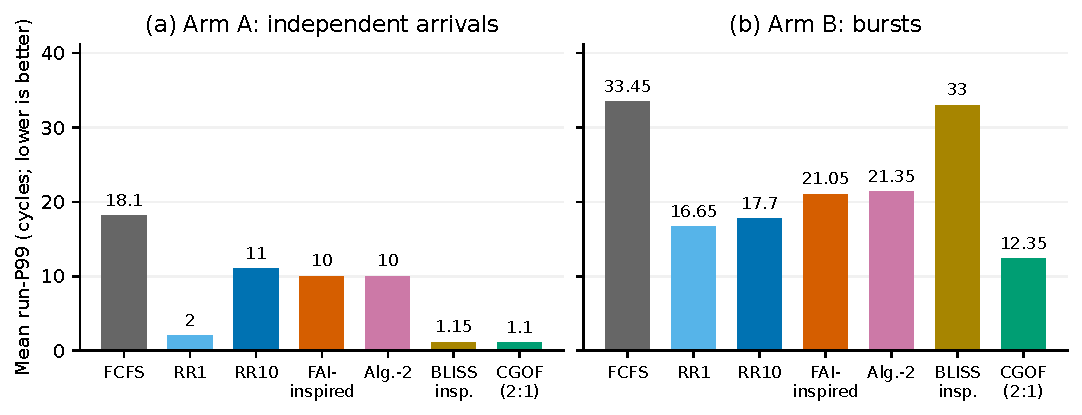
\includegraphics[width=\textwidth]{generated/figures/confirmation.pdf}
\caption{RTL confirmation: mean per-run Sparse generation-to-fire P99 in cycles, twenty seeds 529--548, N4/D16, W5M, after two training windows. A uses independent arrivals and B uses bursts. Individual-policy bars show descriptive means; paired contrast intervals are reported in the text. CGOF (2:1) assigns credits per source.}
\label{fig:confirmation-v3}
\end{figure*}

\begin{figure*}[t]
\centering
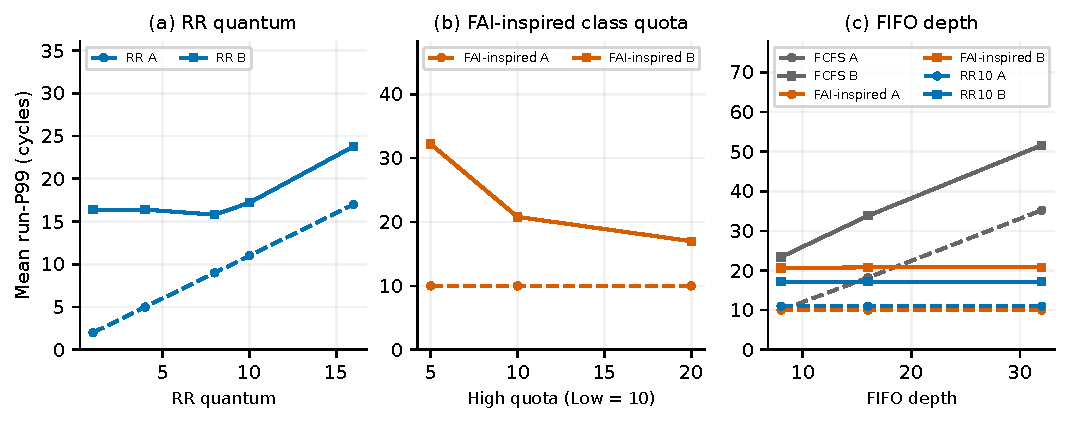
\includegraphics[width=\textwidth]{generated/figures/sensitivity.pdf}
\caption{RTL single-factor sensitivity, five exploration seeds 509--513, no CI. Mean per-run Sparse P99 is in cycles. RR quantum, Main High quota with Low fixed at ten, and FIFO depth are varied separately under the trained A/B method. Curves connect tested settings.}
\label{fig:sensitivity-v3}
\end{figure*}

\begin{figure*}[t]
\centering
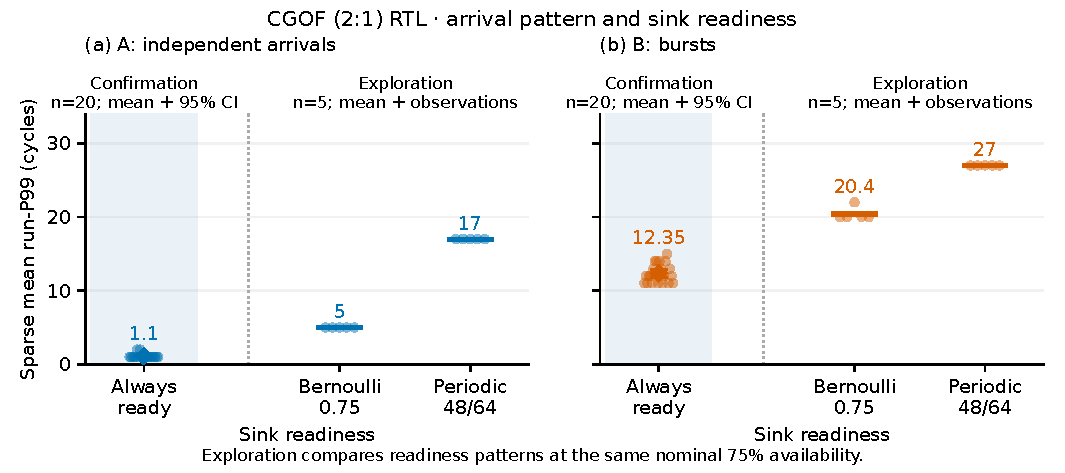
\includegraphics[width=\textwidth]{generated/figures/update-20261029/readiness-confirmation.pdf}
\caption{Current-source CGOF (2:1) RTL replay, N4/D16/W5M after two training windows. Sparse generation-to-fire P99 is averaged within each cohort. Always-ready uses twenty repeated confirmation seeds 529--548 and pointwise bootstrap 95\% CIs; Bernoulli 0.75 and periodic 48/64 readiness each use five exploration seeds 509--513 with descriptive means. A and B retain their independent-arrival and burst definitions. The readiness cohorts have different seed counts and inference status.}
\label{fig:readiness-update}
\par\vspace{8pt}
\centering\small
\setlength{\tabcolsep}{4pt}
\UpdatePerformanceTable
\captionof{table}{Current-source CGOF replay endpoints. Thirty RTL runs yield sixty A/B endpoints: forty always-ready confirmation endpoints and twenty readiness-exploration endpoints. Intervals apply to the twenty-seed confirmation means; exploration is descriptive. This replay uses the original seeds and CGOF only.}
\label{tab:performance-update}
\end{figure*}

\begin{figure*}[t]
\centering
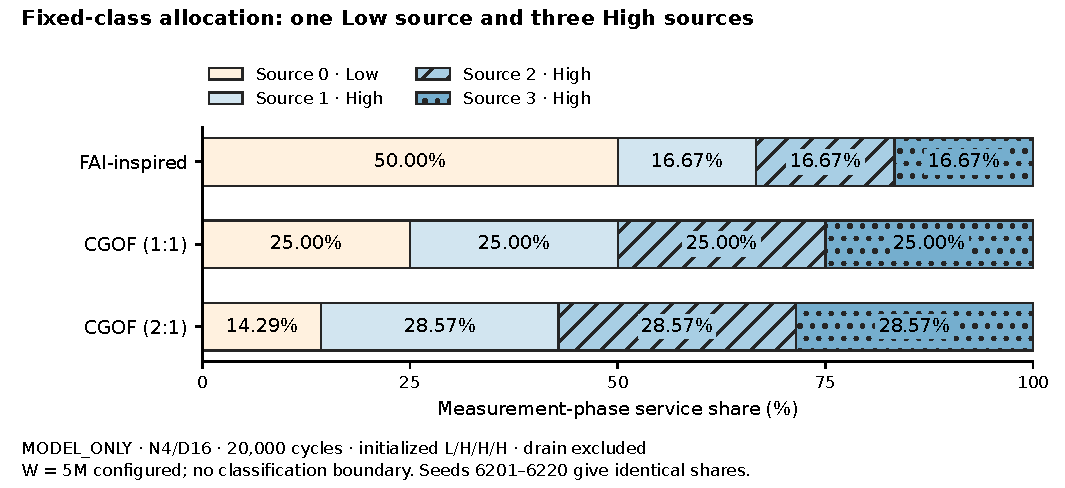
\includegraphics[width=\textwidth]{generated/figures/improvement/allocation-shares.pdf}
\caption{Model allocation at N4/D16, W5M configured: initial Low/High/High/High classes, equal demand, and continuous backlog over 20,000 cycles, before any classification boundary. Main splits class opportunities 10/10; CGOF splits opportunities by source weight. The twenty seeds 6201--6220 yield deterministic endpoints under this control.}
\label{fig:allocation}
\par\vspace{8pt}
\centering\small
\setlength{\tabcolsep}{5pt}
\ImprovementFixedClassTable
\captionof{table}{Measured fixed-class model shares in source order Low/High/High/High, expressed as percentages. Fixed classes and sustained backlog isolate the allocation rule; small deviations from the rational targets reflect the finite observation interval.}
\label{tab:fixed-class}
\end{figure*}

\begin{figure*}[t]
\centering
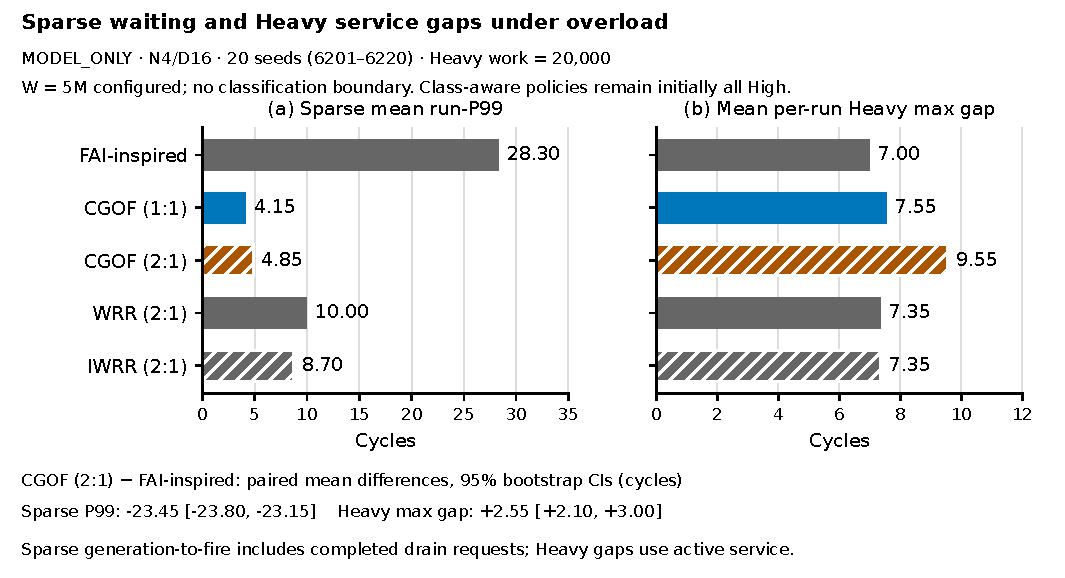
\includegraphics[width=\textwidth]{generated/figures/improvement/heavy-sparse-tradeoff.pdf}
\caption{Model overload at N4/D16 with W5M configured, twenty seeds 6201--6220 and 20,000 Heavy requests. Sparse values average each run's pooled-Sparse generation-to-fire P99; Heavy values average each run's maximum uncensored FIFO-nonempty inter-service wall-cycle gap. Runs finish before the first classification boundary and retain initial all-High classes. Both panels use scheduler cycles with independent axis scales.}
\label{fig:tradeoff}
\par\vspace{8pt}
\centering\small
\setlength{\tabcolsep}{5pt}
\ImprovementFiniteHeavyModelTable
\captionof{table}{Finite-Heavy model overload, N4/D16/W5M configured, twenty paired seeds, 20,000 Heavy requests. Sparse tail is mean per-run generation-to-fire P99; maximum Heavy gap is the mean of run maxima, both in cycles. Completion compares active cycles through Heavy completion in mixed and isolated runs. These jobs finish before the first W5M boundary and retain their initial all-High class map.}
\label{tab:finite-model}
\end{figure*}

\begin{figure*}[t]
\centering\small
\setlength{\tabcolsep}{4pt}
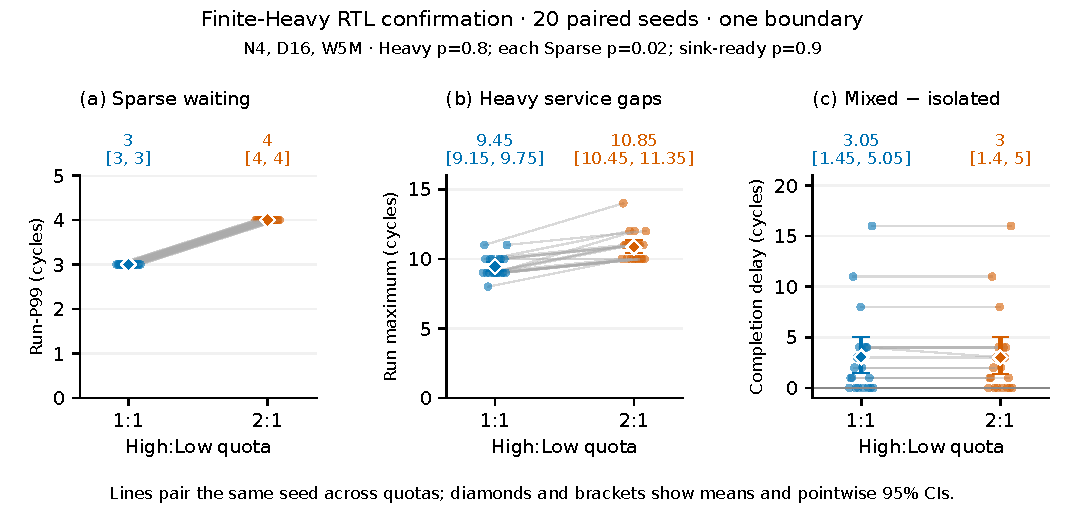
\includegraphics[width=\textwidth]{generated/figures/update-20261029/finite-heavy-confirmation.pdf}
\caption{Finite-Heavy RTL confirmation, N4/D16/W5M, near-load profile, twenty paired seeds 529--548 and five million Heavy requests per run. Both CGOF settings cross one classification boundary. Sparse values are mean per-run generation-to-fire P99; Heavy maxima average uncensored FIFO-nonempty wall-cycle gap maxima. Completion compares mixed with isolated active-cycle totals. Error bars report bootstrap 95\% CIs. Panels use distinct scales and metrics; this near-load RTL cohort is separate from the model overload cohort in Figure~\ref{fig:tradeoff}.}
\label{fig:finite-confirmation}
\par\vspace{8pt}
\UpdateFiniteHeavyTable
\captionof{table}{Twenty-seed finite-Heavy RTL confirmation: eighty runs and forty mixed/isolated pairs across two quota settings. Waiting and gap values use scheduler cycles; completion ratios and mean extra completion cycles compare each mixed run with its paired isolated run. Pointwise 95\% CIs summarize seeds, and paired quota effects are reported in the text.}
\label{tab:finite-rtl}
\end{figure*}

\begin{figure*}[t]
\centering\footnotesize
\setlength{\tabcolsep}{4pt}
\RevisionPrimaryAreaTable
\captionof{table}{N4 complete cell-area decomposition from the primary leaf audit. Descriptor storage, timestamps, policy logic, and common logic are disjoint bins; the residual records report precision. Units are library cell-area units under the common SAED32 TT/25\,ns profile.}
\label{tab:primary-area-v3}
\end{figure*}

\begin{figure*}[t]
\centering
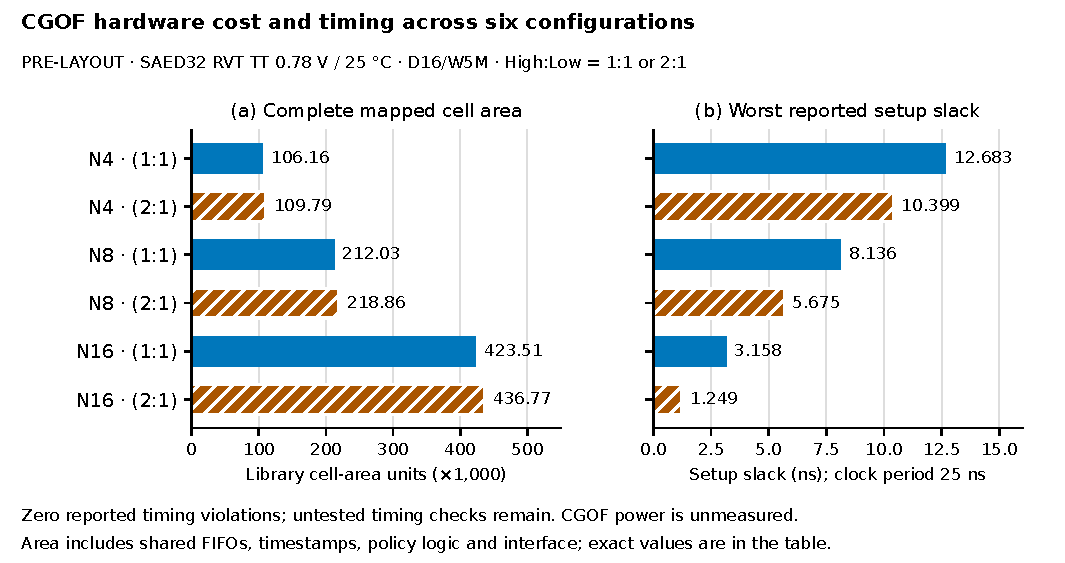
\includegraphics[width=\textwidth]{generated/figures/improvement/cgof-hardware.pdf}
\caption{Six complete CGOF pre-layout mappings, D16/W5M, SAED32 RVT TT 0.78\,V/25$^{\circ}$C and 25\,ns period. Area uses library cell-area units; timing uses reported slack in ns. N8/N16 hardware feasibility is measured independently of behavioral confirmation at those source counts.}
\label{fig:cgof-hardware}
\par\vspace{8pt}
\centering\small
\setlength{\tabcolsep}{5pt}
\ImprovementCgofHardwareTable
\captionof{table}{Complete CGOF area and STA through October 28. All six mappings report zero timing violations at 25\,ns; constant-disabled checks remain disclosed in the raw coverage reports. For 1:1, mapped proofs establish observable-boundary equivalence with 138/230/414 matched unread accounting flip-flops and 8/16/32 unmatched unread reference points at N4/N8/N16. CGOF power is unmeasured.}
\label{tab:cgof-hardware}
\end{figure*}

\subsection{Complete Hardware and Implementation Checks}
Power, performance, and area (PPA) refer respectively to activity-based power estimates, hardware timing, and library cell area. Queueing latency is measured separately. Synthesis and static timing analysis (STA) use Design Compiler and PrimeTime W-2024.09 with the SAED32 32\,nm regular-threshold-voltage (RVT) library at typical--typical (TT), 0.78\,V and 25$^{\circ}$C, with a 25\,ns clock. The shared profile fixes wire-load assumptions, setup/hold uncertainty, I/O delays, and load. Complete costs include descriptors, necessary timestamps, policy state, and common control. These are single-corner pre-layout measurements; routing and clock-tree effects remain outside the measured implementation boundary.

Independent Python models and cocotb scoreboards check cycle-level transfers, ordering, conservation, thresholds, and stalled grants. The completed CGOF matrix contains 463 tests plus 17 separate model unit tests. Source-bound RTL-to-netlist proofs support the mapped comparisons. Primary trained-power estimates use three seeds per policy and zero-delay mapped activity with ideal clocks and no Standard Delay Format (SDF) back-annotation. Static-pin table-range qualifications remain attached to FCFS/RR estimates. Detailed manifests, source bridges, timing coverage, and raw reports are retained with the project evidence~\cite{artifact}.

\section{Results, Mechanism Diagnosis, and Applicability}
\label{sec:results}
\subsection{Queueing Behavior Across Policies and Loads}
Main improves Sparse tail relative to FCFS in both confirmation arms (Figure~\ref{fig:confirmation-v3}). A falls from 18.10 to 10.00 cycles and B from 33.45 to 21.05. RR10 reaches 11.00/17.70, so Main's burst disadvantage is 3.35 cycles, with paired 95\% CI $[2.25,4.45]$. RR1 reaches 2.00/16.65. \Alg{} gives 10.00/21.35, while BLISS-inspired gives 1.15/33.00: excellent independent-arrival behavior can coexist with a substantially higher burst tail.

CGOF (2:1) reaches 1.10/12.35 cycles. Its paired differences from Main are $-8.90$ cycles in A, CI $[-9.00,-8.75]$, and $-8.70$ in B, CI $[-9.50,-7.90]$; all twenty seeds improve in each arm. The policy therefore changes the measured waiting distribution even though the output's service capacity is fixed. In the five-seed N8/N16 exploration, Main's B tail remains above RR10: 27.60/34.80 versus 21.00/24.40. Fan-in changes aggregate Sparse demand and total queue storage together, so these are within-N policy comparisons.

The current-source CGOF replay reproduces the 1.10/12.35-cycle means on the same twenty confirmation seeds (Figure~\ref{fig:readiness-update}, Table~\ref{tab:performance-update}). Its pointwise 95\% intervals are $[1.00,1.25]$ for A and $[11.80,12.90]$ for B. These repeated inputs test reproducibility; they leave the independent seed count at twenty. The replay executes CGOF alone, so the accepted paired Main contrasts above retain their original experimental provenance.

Exploratory sensitivity analysis shows how arbitration parameters affect waiting (Figure~\ref{fig:sensitivity-v3}). Increasing Main's High quota from 5 to 10 to 20 lowers exploratory B P99 from 32.2 to 20.8 to 17.0 cycles, while A remains at ten. Changing depth from 8 to 16 to 32 raises FCFS's A tail from 10.0 to 18.2 to 35.2; Main remains at ten and RR10 at eleven. Under burst stress with 32-request bursts, Main's B tail reaches 88.8 cycles versus 74.4 for RR10 and 87.0 for FCFS. Accepted readiness exploration yields Main and CGOF A/B tails of 17.2/32.6 and 5.0/20.4 under Bernoulli-ready 0.75, and 26.0/34.0 and 17.0/27.0 under periodic 48/64 readiness. The current-source CGOF replay reproduces both readiness means. Both patterns have nominal readiness 0.75, with small differences in realized ready fractions. Their observed Sparse tails differ, supporting measurement of the readiness pattern alongside its average. These five-seed descriptions remain separate from the twenty-seed always-ready confirmation.

A production replay of seed 509 explains one trained-B mechanism. The class map is already Low/High/High/High, and Sparse FIFO-full events are absent. Seven High visits expire with High requests still queued. Fixed-visit offline reorderings of those opportunities fail the tested improvement objective. Together, these observations motivate examining the allocation unit rather than attributing the burst reversal solely to delayed classification.

\subsection{Class Quotas and Per-Source Shares}
\label{sec:allocation}

With both classes continuously active, Main gives each class half the service. A singleton Low source therefore obtains approximately one half, while each of three symmetric High sources obtains one sixth. CGOF (1:1) instead yields one quarter per source; CGOF (2:1) yields $1/7$ for Low and $2/7$ for each High. Figure~\ref{fig:allocation} and Table~\ref{tab:fixed-class} show the measured counterparts. These relations follow from fixed classes, sustained backlog, and complete quota rounds. The labels alone do not determine per-source share.

The class trajectory determines which sources compete under each weight. In the three-window common-demand RTL experiment, bounded saturated producers stop emitting new events when a source has 256 generated-but-unaccepted requests; acceptance frees capacity. Both CGOF settings record measurement fires of 3,750,000/3,750,000/3,750,000/3,749,999. The first boundary is $B_H/B_H/B_H/H$: all four sources remain \emph{effectively High}. The second and third boundaries are $H/H/H/H$. Both settings deliver nearly equal shares under this sustained backlog, with no mixed effective-class competition. Equal weights among active sources explain the share symmetry; intermittent activity can still distinguish one-credit and two-credit rounds. After drain, generated, accepted, and fired totals each equal 15,001,085. Every source has generation-to-fire P99 of 1,086 cycles, with substantial waiting in the bounded external producer backlog.

The short all-High model control likewise yields approximately one quarter for Main, FCFS, RR10, and both CGOF settings. Fixed WRR/IWRR weights $(2,1,1,1)$ target 40/20/20/20\%, a different assignment from CGOF's fixed Low/High example. Weighted Jain is near one for these controls even though raw Jain is about 0.893. Under continuous backlog, oldest-first and eligible round-robin have identical endpoints, whereas predecision quota-compliance accounting requires every source's local FIFO to remain nonempty on every cycle of an active window.

To separate quota from eligible-source ordering under intermittent arrivals, two preregistered RTL campaigns cross High:Low quotas Q1 ($1:1$) and Q2 ($2:1$) with oldest-first (OF) and eligible-round-robin (RR) selection under bursty 90\% readiness (Figure~\ref{fig:followup-20261102}a, Table~\ref{tab:nov-ordering}). In the twenty-seed W256 confirmation (seeds 6501--6520, 160 RTL jobs, 80 mixed/isolated pairs), every seed crosses one active boundary while remaining effectively High. The Q1 ordering delta $d_1=\mathrm{S(Q1,RR)}-\mathrm{S(Q1,OF)}$ is zero in 20/20 seeds; the Q2 ordering delta $d_2$ and the quota-by-ordering interaction $I=d_2-d_1$ are $-1$ cycle in 7/20 seeds and zero in 13/20 (mean $-0.35$, median $0$). Because the frozen gate required at least 15/20 joint strict improvements, the primary superiority claim is \code{NOT\_CONFIRMED}. In the separate five-seed W5M production exploration (seeds 6601--6605, 40 RTL jobs, 20 pairs, 5M Heavy requests per job), every seed crosses the sole active boundary at cycle 4,999,999 ($H/H/H/H\rightarrow B_H/H/H/H$) and finishes near 6.25M cycles with matched Sparse cohorts and zero censoring. All five seeds yield mixed Sparse P99 of $S=11/11/12/11$ cycles across Q1-OF, Q1-RR, Q2-OF, and Q2-RR ($d_1=0$, $d_2=-1$, $I=-1$). However, RR increases the Q1 mixed Heavy maximum wall gap by $+2,+2,+1,+2,+1$ cycles (mean $+1.6$) while Q2 changes by $0,0,0,0,-1$ (mean $-0.2$). Extra Heavy completion delay $A=C_{\rm mixed}-C_{\rm isolated}$ is identical across all four settings within each seed ($3,0,7,1,8$ cycles; RR minus OF is $0$ in 10/10 comparisons). Eligible RR thus trades a one-cycle Q2 Sparse P99 reduction against a larger Q1 worst-case Heavy gap, establishing a descriptive tradeoff rather than a universal winner.

\subsection{Sparse Gains and Heavy Service Regularity}

Finite-work experiments distinguish total completion from short-term service regularity. In the model overload cohort, Main's Sparse P99 is 28.30 cycles; CGOF (1:1) and (2:1) reduce it to 4.15 and 4.85 (Table~\ref{tab:finite-model}). The mean maximum Heavy gap rises from 7.00 to 7.55 and 9.55. CGOF (2:1) minus Main gives $-23.45$ cycles for Sparse P99, CI $[-23.80,-23.15]$, and $+2.55$ for maximum Heavy gap, CI $[2.10,3.00]$. WRR and IWRR reach Sparse P99 of 10.00 and 8.70 with Heavy maximum gap 7.35, providing intermediate operating points.

The completion ratios tell a different story: Main is 1.2002146, CGOF (1:1) 1.2004486, and CGOF (2:1) 1.2004373. The CGOF (2:1) difference is $+0.0002227$, accompanied by a Heavy throughput-ratio difference of $-0.0001544$. The large Sparse-tail reduction is accompanied by a much smaller increase in total Heavy completion duration in this workload.

The twenty-seed production RTL confirmation separates these effects directly (Figure~\ref{fig:finite-confirmation}, Table~\ref{tab:finite-rtl}). CGOF (1:1)/(2:1) gives Sparse P99 of 3/4 cycles and mean per-run maximum Heavy gap of 9.45/10.85 cycles. The paired 2:1-minus-1:1 changes are $+1.00$ Sparse-P99 cycle, CI $[1.00,1.00]$, and $+1.40$ maximum-gap cycles, CI $[1.10,1.75]$. Heavy wall-gap P99 remains three cycles for both settings. Thus the upper extreme changes while this percentile remains fixed.

\begin{figure*}[t]
\centering\small
\setlength{\tabcolsep}{4pt}
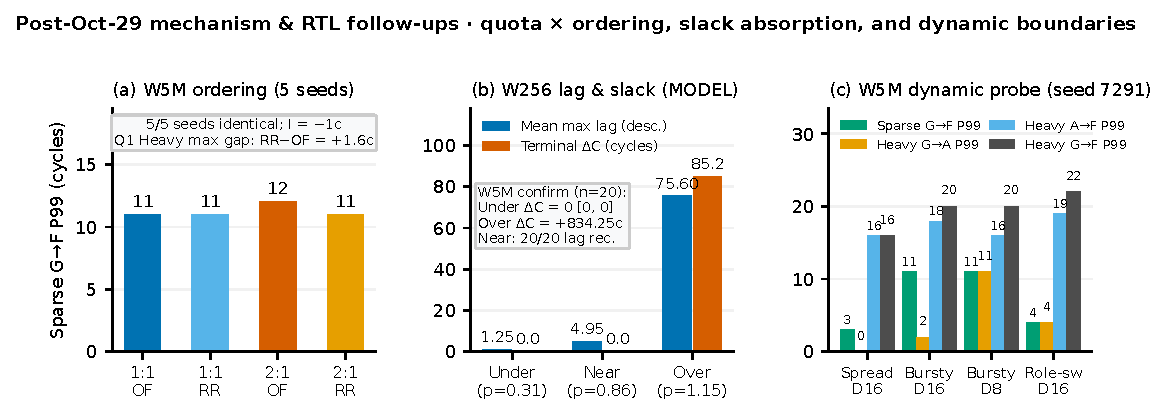
\includegraphics[width=\textwidth]{generated/figures/update-20261102/followup-synthesis-20261102.pdf}
\caption{Post-October-29 mechanism and RTL follow-up synthesis: (a) five-seed W5M production quota-by-ordering descriptive exploration (seeds 6601--6605, 40 RTL jobs); (b) MODEL\_ONLY arrival-phase spare-capacity absorption (20 confirmation seeds 6201--6220 at W5M) and common-horizon transient lag recovery (5 exploration seeds $\times$ 4 phases at W256); (c) single-seed four-window W5M dynamic RTL probe (seed 7291, 20 RTL jobs, CI null) across readiness arrangements, role switching, and D8/D16 admission boundaries.}
\label{fig:followup-20261102}
\par\vspace{6pt}
\footnotesize
\NovOrderingTable
\captionof{table}{Quota-by-ordering RTL campaigns under bursty 90\% readiness (N4/D16, near load). W256 confirmation ($n=20$ seeds, 160 jobs) tests joint $d_2\le -1, I\le -1$ against a 15/20 gate (\code{NOT\_CONFIRMED}). W5M production ($n=5$ seeds, 40 jobs) is a descriptive exploration across 5M Heavy requests per job.}
\label{tab:nov-ordering}
\par\vspace{6pt}
\NovArrivalSlackTable
\captionof{table}{MODEL\_ONLY spare-capacity absorption and common-generation-horizon transient Heavy lag recovery. W5M confirmation ($n=20$ seeds 6201--6220) reports 10,000-replicate paired bootstrap 95\% CIs against a predeclared $\pm 20$-cycle completion margin; W256 P0 screening ($5$ seeds $\times 4$ phases) tracks post-edge Heavy fire lag $\mathrm{lag}(k)=F_{\rm isolated}(k)-F_{\rm mixed}(k)$ under scenario-ready drain.}
\label{tab:nov-slack}
\end{figure*}

For CGOF (1:1) and (2:1), the mean mixed/isolated completion ratios are 1.000000488 and 1.000000480, respectively. Mixed completion requires an average of 3.05 and 3.00 additional cycles, with CIs $[1.45,5.05]$ and $[1.40,5.00]$. The paired quota effect on completion ratio is approximately $-8.0\times10^{-9}$, CI $[-2.40\times10^{-8},0]$, while the mean extra-cycle effect is $-0.05$ cycle. The near profile's nominal offered rate is $0.80+3(0.02)=0.86$ requests per cycle against 0.90 ready probability. A twenty-seed W5M \code{MODEL\_ONLY} confirmation (seeds 6201--6220, 80 pairs) and a 120-pair W256 common-generation-horizon screen test how spare service capacity governs this completion behavior (Figure~\ref{fig:followup-20261102}b, Table~\ref{tab:nov-slack}). Under W5M under-load, mixed-minus-isolated Heavy completion delay is $0.00$ cycles, CI $[0.0,0.0]$, with 20/20 seeds inside the predeclared 20-cycle equivalence margin; under over-load, it rises to $+834.25$ cycles, CI $[820.4,849.3]$ (ratio $1.037553$), with 0/20 inside the margin. Under the repaired P0 common-generation contract—which continues emitting declared Sparse work through horizon $H$ and drains under the scenario's own readiness trace—near-load execution incurs a mean maximum transient lag of $5.00/4.95$ Heavy descriptors for CGOF (1:1)/(2:1), yet 20/20 observations recover to zero terminal completion delta before cutoff. Spare service opportunities therefore absorb Sparse work below capacity, whereas overload converts Sparse protection into an explicit Heavy completion cost. Sparse-only Jain is approximately 0.999994 for both settings in the near-load RTL confirmation, and Heavy accounts for approximately 93.023\% of mixed service.

For this near-load quota comparison, 1:1 has both the lower Sparse P99 and the smaller mean maximum Heavy gap. The 2:1 setting's mean extra completion time is only 0.05 cycle lower. The result therefore identifies a finer service round with better measured temporal regularity at this operating point. The Sparse benefit accompanied by a Heavy-gap cost appears in the separate model comparison of Main with CGOF under overload.

Each mixed run crosses a boundary with $B_H/H/H/H$, retaining effective High for every source. The 2:1 setting therefore gives each source two credits per refill, compared with one under 1:1. Their relative weights are equal, but a source may use its second credit before the next refill. Under intermittent activity, this changes the available credits encountered by later arrivals. A deterministic \code{MODEL\_ONLY} credit-refill trace (\code{cxl-credit-refill-trace-v2}) holds arrivals, stalls, and all-High classes fixed while changing only the per-source High credit from 1 to 2, separating live candidate state, latched offered grants across stalls, and committed fire snapshots. Across five Sparse arrival-phase shifts, three shifts diverge at cycle 4 or 7—two via refill timing and one via eligibility—while two shifts show no divergence, confirming that absolute credit budgets alter short-term service order through refill and eligibility phase.

Figure~\ref{fig:tradeoff} compares policies under model overload; Figure~\ref{fig:finite-confirmation} compares CGOF budgets under near-load RTL execution. Their controls and loads establish complementary pieces of the service-regularity argument. The earlier trained RTL confirmation also shows why a single Heavy metric is insufficient: in arm B, CGOF (2:1) lowers the maximum across runs of the maximum wall gap from 11 to 7 while gap P99 rises from 1 to 3. A lower extreme can coexist with more frequent moderate gaps. Buffer adaptation introduces another timescale: retained-state role switches change Main's effective classes after 10M cycles versus 5M for \Alg, but earlier classification did not improve whole-role Sparse waiting in that experiment. Two separate \code{MODEL\_ONLY} Buffer screens further isolate transition mechanics from closed-loop queueing without claiming latency recovery. In 78 transition-only replays per window across phases $0,64,255$, Main filters a one-window noise pulse with zero effective flips versus two flips for single-window Main-1W and \Alg, while persistent role changes settle in $448\text{--}704$ cycles for Main versus $192\text{--}448$ for Main-1W at W256 (depending on mixed-window B/S evidence rather than a fixed $2W$ constant). In 720 closed-loop W256 runs across seeds 6101--6105, CGOF (1:1) matches identically across live, 1W, and frozen all-High classifiers in 120/120 scenario groups (negative control PASS), whereas CGOF (2:1) shows that classifier settle delay and generation-cohort waiting P99 vary in distinct directions.

Finally, an exploratory single-seed W5M dynamic RTL probe (seed 7291, 20 RTL runs, 10 mixed/isolated pairs, \code{confidence\_intervals: null}; Figure~\ref{fig:followup-20261102}c) exercises four active W5M classification boundaries across 17.5M Heavy requests per run. Static-role runs transition $H/H/H/H\rightarrow B_H/H/H/H\rightarrow L/H/H/H$; physical role switching $[0,0,1,1]$ induces three effective class transitions while preserving generation-role conservation. At nearly identical 90\% realized readiness ($0.89999999$ vs.\ $0.90000011$), clustering stalls into bursty intervals raises both Sparse G$\rightarrow$F P99 and Heavy wall-gap P99 from 3 to 11 cycles while Heavy ready-opportunity gap P99 stays 2. Reducing FIFO depth from D16 to D8 under bursty readiness leaves total Heavy G$\rightarrow$F P99 at 20 cycles and Sparse P99 at 11 cycles, but shifts Heavy waiting from post-admission queueing ($A\rightarrow F$ P99 from 18 to 16) to pre-admission backlog ($G\rightarrow A$ P99 from 2 to 11).

\subsection{Complete Hardware Cost}

Complete hardware cost makes the price of ordering visible. At N4, FCFS, RR10, and Main occupy 103,970.058, 79,047.172, and 110,089.846 library cell-area units. Across N4/N8/N16, Main is 38.22--39.27\% larger than RR10. Table~\ref{tab:primary-area-v3} separates descriptor and timestamp storage from policy and common logic. At N16, the 256 entries contain 26,880 descriptor bits; FCFS and Main additionally require 8,192 timestamp bits. RR's lower cost reflects both simpler arbitration and the absence of ordering metadata.

The six CGOF configurations meet evaluated setup and hold checks (Figure~\ref{fig:cgof-hardware}, Table~\ref{tab:cgof-hardware}). For 1:1, area grows from 106,163.066946 at N4 to 423,513.448454 at N16; corresponding 2:1 areas are 109,794.784709 and 436,771.124393. N16 setup margins are 3.158005 and 1.248813\,ns. At N4, CGOF (2:1) differs from Main by $-0.268019\%$ in whole-design area and adds three registers. Top-level glue contributes part of this small difference. Thus the measured tail benefit is available at a complete cost close to Main under this mapping profile.

The 1:1 configuration also illustrates the connection between semantics and synthesis: equal class weights make classifier outputs irrelevant to observable selection, permitting dead-state optimization. Its proof scope therefore follows observable behavior with the disclosed unread accounting and optimized-away reference state. N4 CGOF (2:1) passes all 9,126 compare points. Timing retains constant-disabled checks, and the wire-load clock-fanout cap can make absolute pre-layout estimates optimistic; the reported margins characterize the common constrained flow.

Baseline trained-power A/B means are 3.356/3.356\,mW for FCFS, 2.559667/2.560000 for RR10, and 3.466667/3.466000 for Main. These three-seed estimates use the activity and warning qualifications in Section~\ref{sec:method}. CGOF's area and timing measurements leave its power comparison open.

\balance
\subsection{Applicability and Next Questions}
These results support selecting a policy according to the required service behavior and hardware budget. RR provides a relatively small implementation with competitive measured burst tails when timestamp storage and dynamic classification are unnecessary. Across the three specified objectives and measured scope—Sparse tail protection, per-source fairness under asymmetric class cardinality, and complete pre-layout hardware cost—CGOF provides the strongest overall operating point, without claiming an unconditional Pareto-optimal or universal winner across every metric: at nearly identical N4 area to Main ($-0.268\%$ for 2:1 and $-3.567\%$ for 1:1), it eliminates single-Low class-quota skew and reduces trained Sparse P99 by 41--89\% relative to Main, while subject to three explicit boundaries: (i) under overload contention it trades 1--2.55 additional cycles of worst-case Heavy inter-service gap while preserving long-run Heavy completion and throughput; (ii) when arrival-order timestamps and dynamic classification are not required, RR10 occupies 24--28\% less cell area; and (iii) in the single-boundary all-effective-High near-load RTL confirmation, CGOF (1:1) yields a lower Sparse tail (3 vs.\ 4 cycles) and smaller maximum Heavy gaps (9.45 vs.\ 10.85 cycles) than CGOF (2:1). Relative source weights specify the fixed-class allocation target, while absolute budgets and eligible ordering shape short-term service regularity under intermittent demand.

The completed follow-up evidence separates confirmed scheduler-boundary effects from descriptive and model-scoped mechanisms. The twenty-seed W256 ordering confirmation (\code{NOT\_CONFIRMED}) and five-seed W5M production exploration show that eligible round-robin ordering modifies Sparse P99 by at most one cycle in Q2 while raising Q1 worst-case Heavy gaps, confirming that per-source credit allocation rather than intra-eligible ordering is the primary lever. The twenty-seed W5M model confirmation and common-horizon lag screen establish spare-capacity absorption below saturation, while the single-seed four-window RTL probe demonstrates multi-boundary transitions, bursty-stall amplification, and D8 admission-wait shifting. Remaining work outside the present confirmed RTL scope includes multi-seed W5M dynamic role-switch and under/over RTL confirmation, explicit latency-recovery horizon evaluation, CGOF gate-level SAIF power, and calibrated CXL system integration measuring issue-to-response latency, completed bytes, and application slowdown. The present evidence establishes a reproducible, source-bound relationship among service classes, allocation units, waiting distributions, and complete hardware cost for an equal-cost, single-output switch.

\paragraph{AI use acknowledgment.}
Claude Code with RTL Agent Team and GPT-6.1 Sol assisted implementation and verification. GPT-6.1 Sol/high assisted manuscript drafting, evidence review, and figure production; Gemini 3.8 Flash/high reviewed language. Codex coordinated source verification, selective editorial integration, and PDF acceptance. Numerical claims derive from the archived experiments and reports. The authors retain responsibility for the interpretation and final text.

\clearpage

\begingroup\footnotesize\balance
\begin{thebibliography}{99}
\bibitem{cxl_intro} D. Das Sharma, R. Blankenship, and D. Berger, ``An Introduction to the Compute Express Link (CXL) Interconnect,'' \emph{ACM Computing Surveys}, vol.~56, no.~11, pp.~1--37, 2024. doi: \href{https://doi.org/10.1145/3669900}{10.1145/3669900}.
\bibitem{pond} H. Li \emph{et al.}, ``Pond: CXL-Based Memory Pooling Systems for Cloud Platforms,'' arXiv:2203.00241v4, October 21, 2022. ASPLOS 2023 preprint; version used here. \href{https://arxiv.org/abs/2203.00241v4}{arXiv:2203.00241v4}.
\bibitem{tpp} H. Al Maruf \emph{et al.}, ``TPP: Transparent Page Placement for CXL-Enabled Tiered-Memory,'' in \emph{Proc. 28th ACM Int. Conf. Architectural Support for Programming Languages and Operating Systems}, vol.~3, 2023, pp.~742--755. doi: \href{https://doi.org/10.1145/3582016.3582063}{10.1145/3582016.3582063}.
\bibitem{directcxl} D. Gouk, M. Kwon, H. Bae, S. Lee, and M. Jung, ``Memory Pooling With CXL,'' \emph{IEEE Micro}, vol.~43, no.~2, pp.~48--57, 2023. doi: \href{https://doi.org/10.1109/MM.2023.3237491}{10.1109/MM.2023.3237491}.
\bibitem{case_pool} P. Levis, K. Lin, and A. Tai, ``A Case Against CXL Memory Pooling,'' in \emph{Proc. 22nd ACM Workshop on Hot Topics in Networks}, 2023, pp.~18--24. doi: \href{https://doi.org/10.1145/3626111.3628195}{10.1145/3626111.3628195}.
\bibitem{my_cxl_pool} Y. Zhong \emph{et al.}, ``My CXL Pool Obviates Your PCIe Switch,'' in \emph{Proc. Workshop on Hot Topics in Operating Systems}, 2025, pp.~58--66. doi: \href{https://doi.org/10.1145/3713082.3730393}{10.1145/3713082.3730393}.
\bibitem{stfm} O. Mutlu and T. Moscibroda, ``Stall-Time Fair Memory Access Scheduling for Chip Multiprocessors,'' in \emph{Proc. 40th IEEE/ACM Int. Symp. Microarchitecture}, 2007, pp.~146--160. doi: \href{https://doi.org/10.1109/MICRO.2007.21}{10.1109/MICRO.2007.21}.
\bibitem{fqmem} K. J. Nesbit, N. Aggarwal, J. Laudon, and J. E. Smith, ``Fair Queuing Memory Systems,'' in \emph{Proc. 39th IEEE/ACM Int. Symp. Microarchitecture}, 2006, pp.~208--222. doi: \href{https://doi.org/10.1109/MICRO.2006.24}{10.1109/MICRO.2006.24}.
\bibitem{atlas} Y. Kim, D. Han, O. Mutlu, and M. Harchol-Balter, ``ATLAS: A Scalable and High-Performance Scheduling Algorithm for Multiple Memory Controllers,'' in \emph{Proc. 16th IEEE Int. Symp. High-Performance Computer Architecture}, 2010, pp.~1--12. doi: \href{https://doi.org/10.1109/HPCA.2010.5416658}{10.1109/HPCA.2010.5416658}.
\bibitem{tcm} Y. Kim, M. Papamichael, O. Mutlu, and M. Harchol-Balter, ``Thread Cluster Memory Scheduling: Exploiting Differences in Memory Access Behavior,'' in \emph{Proc. 43rd IEEE/ACM Int. Symp. Microarchitecture}, 2010, pp.~65--76. doi: \href{https://doi.org/10.1109/MICRO.2010.51}{10.1109/MICRO.2010.51}.
\bibitem{bliss} L. Subramanian, D. Lee, V. Seshadri, H. Rastogi, and O. Mutlu, ``The Blacklisting Memory Scheduler: Achieving High Performance and Fairness at Low Cost,'' in \emph{Proc. IEEE 32nd Int. Conf. Computer Design}, 2014, pp.~8--15. doi: \href{https://doi.org/10.1109/ICCD.2014.6974655}{10.1109/ICCD.2014.6974655}.
\bibitem{fai} J. Li, Y. Liu, Y. Gu, and C. Wu, ``FAI-CXL: An Efficient Hardware-Accelerated Fairness-Aware CXL Memory Pool Management with Fine-Grained Cacheline-Level Interleaving,'' in \emph{Proc. IEEE Int. Conf. Parallel and Distributed Systems (ICPADS)}, 2025, pp.~1--8. doi: \href{https://doi.org/10.1109/ICPADS67057.2025.11322896}{10.1109/ICPADS67057.2025.11322896}. Algorithm 2, p.~5.
\bibitem{cxl_interplay} S. Mao \emph{et al.}, ``CXL-INTERPLAY: Unraveling and Characterizing CXL Interference in Modern Computer Systems,'' in \emph{Proc. 62nd ACM/IEEE Design Automation Conference}, 2025, pp.~1--7. doi: \href{https://doi.org/10.1109/DAC63849.2025.11132607}{10.1109/DAC63849.2025.11132607}.
\bibitem{contention_cache} C. Tirumalasetty and N. R. Annapareddy, ``Contention Aware DRAM Caching for CXL-Enabled Pooled Memory,'' in \emph{Proc. Int. Symp. Memory Systems}, 2024, pp.~157--171. doi: \href{https://doi.org/10.1145/3695794.3695808}{10.1145/3695794.3695808}.
\bibitem{hpc_pool} J. Wahlgren, M. Gokhale, and I. B. Peng, ``Evaluating Emerging CXL-Enabled Memory Pooling for HPC Systems,'' in \emph{Proc. IEEE/ACM Workshop on Memory Centric High Performance Computing}, 2022, pp.~11--20. doi: \href{https://doi.org/10.1109/MCHPC56545.2022.00007}{10.1109/MCHPC56545.2022.00007}.
\bibitem{cxldmsim} Y. Wang \emph{et al.}, ``CXL-DMSim: A Full-System CXL Disaggregated Memory Simulator With Comprehensive Silicon Validation,'' \emph{IEEE Trans. Computer-Aided Design of Integrated Circuits and Systems}, vol.~45, no.~4, pp.~1787--1801, 2026. doi: \href{https://doi.org/10.1109/TCAD.2025.3607145}{10.1109/TCAD.2025.3607145}.
\bibitem{gupta} P. Gupta and N. McKeown, ``Designing and Implementing a Fast Crossbar Scheduler,'' \emph{IEEE Micro}, vol.~19, no.~1, pp.~20--28, 1999. doi: \href{https://doi.org/10.1109/40.748793}{10.1109/40.748793}.
\bibitem{wrr_mandal} S. K. Mandal, J. Tong, R. Ayoub, M. Kishinevsky, A. Abousamra, and U. Y. Ogras, ``Theoretical Analysis and Evaluation of NoCs with Weighted Round-Robin Arbitration,'' arXiv:2108.09534v2, August 12, 2023. \href{https://arxiv.org/abs/2108.09534v2}{arXiv:2108.09534v2}.
\bibitem{artifact} J. Chiang and D. Chou, \emph{CXL Scheduler Project: Frozen Specification v1.0 and Experimental Evidence}, ECE 509 project artifact, revised November 2, 2026. Includes source-bound RTL experiments, model diagnosis cohorts, complete area/STA and activity reports, and manuscript-update evidence manifests.
\end{thebibliography}
\endgroup
\end{document}
